\iffalse
\documentclass[journal,12pt,twocolumn]{IEEEtran}
%
\usepackage{setspace}
\usepackage{gensymb}
\usepackage{xcolor}
\usepackage{caption}
%\usepackage{subcaption}
%\doublespacing
\singlespacing

%\usepackage{graphicx}
%\usepackage{amssymb}
%\usepackage{relsize}
\usepackage[cmex10]{amsmath}
\usepackage{mathtools}
%\usepackage{amsthm}
%\interdisplaylinepenalty=2500
%\savesymbol{iint}
%\usepackage{txfonts}
%\restoresymbol{TXF}{iint}
%\usepackage{wasysym}
\usepackage{amsthm}
\usepackage{mathrsfs}
\usepackage{txfonts}
\usepackage{stfloats}
\usepackage{cite}
\usepackage{cases}
\usepackage{subfig}
%\usepackage{xtab}
\usepackage{longtable}
\usepackage{multirow}
%\usepackage{algorithm}
%\usepackage{algpseudocode}
\usepackage{enumitem}
\usepackage{mathtools}
\usepackage{iithtlc}
%\usepackage[framemethod=tikz]{mdframed}
\usepackage{listings}


%\usepackage{stmaryrd}


%\usepackage{wasysym}
%\newcounter{MYtempeqncnt}
\DeclareMathOperator*{\Res}{Res}
%\renewcommand{\baselinestretch}{2}
\renewcommand\thesection{\arabic{section}}
\renewcommand\thesubsection{\thesection.\arabic{subsection}}
\renewcommand\thesubsubsection{\thesubsection.\arabic{subsubsection}}

\renewcommand\thesectiondis{\arabic{section}}
\renewcommand\thesubsectiondis{\thesectiondis.\arabic{subsection}}
\renewcommand\thesubsubsectiondis{\thesubsectiondis.\arabic{subsubsection}}

% correct bad hyphenation here
\hyphenation{op-tical net-works semi-conduc-tor}

\lstset{
language=Python,
frame=single, 
breaklines=true
}

%\lstset{
	%%basicstyle=\small\ttfamily\bfseries,
	%%numberstyle=\small\ttfamily,
	%language=Octave,
	%backgroundcolor=\color{white},
	%%frame=single,
	%%keywordstyle=\bfseries,
	%%breaklines=true,
	%%showstringspaces=false,
	%%xleftmargin=-10mm,
	%%aboveskip=-1mm,
	%%belowskip=0mm
%}

%\surroundwithmdframed[width=\columnwidth]{lstlisting}


\begin{document}
%

\theoremstyle{definition}
\newtheorem{theorem}{Theorem}[section]
\newtheorem{problem}{Problem}
\newtheorem{proposition}{Proposition}[section]
\newtheorem{lemma}{Lemma}[section]
\newtheorem{corollary}[theorem]{Corollary}
\newtheorem{example}{Example}[section]
\newtheorem{definition}{Definition}[section]
%\newtheorem{algorithm}{Algorithm}[section]
%\newtheorem{cor}{Corollary}
\newcommand{\BEQA}{\begin{eqnarray}}
\newcommand{\EEQA}{\end{eqnarray}}
\newcommand{\define}{\stackrel{\triangle}{=}}

\bibliographystyle{IEEEtran}
%\bibliographystyle{ieeetr}

\providecommand{\nCr}[2]{\,^{#1}C_{#2}} % nCr
\providecommand{\nPr}[2]{\,^{#1}P_{#2}} % nPr
\providecommand{\mbf}{\mathbf}
\providecommand{\pr}[1]{\ensuremath{\Pr\left(#1\right)}}
\providecommand{\qfunc}[1]{\ensuremath{Q\left(#1\right)}}
\providecommand{\sbrak}[1]{\ensuremath{{}\left[#1\right]}}
\providecommand{\lsbrak}[1]{\ensuremath{{}\left[#1\right.}}
\providecommand{\rsbrak}[1]{\ensuremath{{}\left.#1\right]}}
\providecommand{\brak}[1]{\ensuremath{\left(#1\right)}}
\providecommand{\lbrak}[1]{\ensuremath{\left(#1\right.}}
\providecommand{\rbrak}[1]{\ensuremath{\left.#1\right)}}
\providecommand{\cbrak}[1]{\ensuremath{\left\{#1\right\}}}
\providecommand{\lcbrak}[1]{\ensuremath{\left\{#1\right.}}
\providecommand{\rcbrak}[1]{\ensuremath{\left.#1\right\}}}
\theoremstyle{remark}
\newtheorem{rem}{Remark}
\newcommand{\sgn}{\mathop{\mathrm{sgn}}}
\providecommand{\abs}[1]{\left\vert#1\right\vert}
\providecommand{\res}[1]{\Res\displaylimits_{#1}} 
\providecommand{\norm}[1]{\lVert#1\rVert}
\providecommand{\mtx}[1]{\mathbf{#1}}
\providecommand{\mean}[1]{E\left[ #1 \right]}
\providecommand{\fourier}{\overset{\mathcal{F}}{ \rightleftharpoons}}
%\providecommand{\hilbert}{\overset{\mathcal{H}}{ \rightleftharpoons}}
\providecommand{\system}{\overset{\mathcal{H}}{ \longleftrightarrow}}
	%\newcommand{\solution}[2]{\textbf{Solution:}{#1}}
\newcommand{\solution}{\noindent \textbf{Solution: }}
\providecommand{\dec}[2]{\ensuremath{\overset{#1}{\underset{#2}{\gtrless}}}}
%\numberwithin{equation}{subsection}
\numberwithin{equation}{problem}
%\numberwithin{problem}{subsection}
%\numberwithin{definition}{subsection}
\makeatletter
\@addtoreset{figure}{problem}
\makeatother

\let\StandardTheFigure\thefigure
%\renewcommand{\thefigure}{\theproblem.\arabic{figure}}
\renewcommand{\thefigure}{\theproblem}


%\numberwithin{figure}{subsection}

\def\putbox#1#2#3{\makebox[0in][l]{\makebox[#1][l]{}\raisebox{\baselineskip}[0in][0in]{\raisebox{#2}[0in][0in]{#3}}}}
     \def\rightbox#1{\makebox[0in][r]{#1}}
     \def\centbox#1{\makebox[0in]{#1}}
     \def\topbox#1{\raisebox{-\baselineskip}[0in][0in]{#1}}
     \def\midbox#1{\raisebox{-0.5\baselineskip}[0in][0in]{#1}}

\vspace{3cm}

\title{ 
\logo{
C and Python 
}
%	\logo{Octave for Math Computing }
}
%\title{
%	\logo{Matrix Analysis through Octave}{\begin{center}\includegraphics[scale=.24]{tlc}\end{center}}{}{HAMDSP}
%}


% paper title
% can use linebreaks \\ within to get better formatting as desired
%\title{Matrix Analysis through Octave}
%
%
% author names and IEEE memberships
% note positions of commas and nonbreaking spaces ( ~ ) LaTeX will not break
% a structure at a ~ so this keeps an author's name from being broken across
% two lines.
% use \thanks{} to gain access to the first footnote area
% a separate \thanks must be used for each paragraph as LaTeX2e's \thanks
% was not built to handle multiple paragraphs
%

\author{G V V Sharma$^{*}$ %<-this  stops a space
\thanks{*The author is with the Department
of Electrical Engineering, Indian Institute of Technology, Hyderabad
502285 India e-mail:  gadepall@iith.ac.in.}% <-this % stops a space
%\thanks{J. Doe and J. Doe are with Anonymous University.}% <-this % stops a space
%\thanks{Manuscript received April 19, 2005; revised January 11, 2007.}}
}
% note the % following the last \IEEEmembership and also \thanks - 
% these prevent an unwanted space from occurring between the last author name
% and the end of the author line. i.e., if you had this:
% 
% \author{....lastname \thanks{...} \thanks{...} }
%                     ^------------^------------^----Do not want these spaces!
%
% a space would be appended to the last name and could cause every name on that
% line to be shifted left slightly. This is one of those "LaTeX things". For
% instance, "\textbf{A} \textbf{B}" will typeset as "A B" not "AB". To get
% "AB" then you have to do: "\textbf{A}\textbf{B}"
% \thanks is no different in this regard, so shield the last } of each \thanks
% that ends a line with a % and do not let a space in before the next \thanks.
% Spaces after \IEEEmembership other than the last one are OK (and needed) as
% you are supposed to have spaces between the names. For what it is worth,
% this is a minor point as most people would not even notice if the said evil
% space somehow managed to creep in.



% The paper headers
%\markboth{Journal of \LaTeX\ Class Files,~Vol.~6, No.~1, January~2007}%
%{Shell \MakeLowercase{\textit{et al.}}: Bare Demo of IEEEtran.cls for Journals}
% The only time the second header will appear is for the odd numbered pages
% after the title page when using the twoside option.
% 
% *** Note that you probably will NOT want to include the author's ***
% *** name in the headers of peer review papers.                   ***
% You can use \ifCLASSOPTIONpeerreview for conditional compilation here if
% you desire.




% If you want to put a publisher's ID mark on the page you can do it like
% this:
%\IEEEpubid{0000--0000/00\$00.00~\copyright~2007 IEEE}
% Remember, if you use this you must call \IEEEpubidadjcol in the second
% column for its text to clear the IEEEpubid mark.



% make the title area
\maketitle

%\newpage

%\tableofcontents


%\begin{abstract}
%%\boldmath
%In this letter, an algorithm for evaluating the exact analytical bit error rate  (BER)  for the piecewise linear (PL) combiner for  multiple relays is presented. Previous results were available only for upto three relays. The algorithm is unique in the sense that  the actual mathematical expressions, that are prohibitively large, need not be explicitly obtained. The diversity gain due to multiple relays is shown through plots of the analytical BER, well supported by simulations. 
%
%\end{abstract}
% IEEEtran.cls defaults to using nonbold math in the Abstract.
% This preserves the distinction between vectors and scalars. However,
% if the journal you are submitting to favors bold math in the abstract,
% then you can use LaTeX's standard command \boldmath at the very start
% of the abstract to achieve this. Many IEEE journals frown on math
% in the abstract anyway.

% Note that keywords are not normally used for peerreview papers.
%\begin{IEEEkeywords}
%Cooperative diversity, decode and forward, piecewise linear
%\end{IEEEkeywords}



% For peer review papers, you can put extra information on the cover
% page as needed:
% \ifCLASSOPTIONpeerreview
% \begin{center} \bfseries EDICS Category: 3-BBND \end{center}
% \fi
%
% For peerreview papers, this IEEEtran command inserts a page break and
% creates the second title. It will be ignored for other modes.
\IEEEpeerreviewmaketitle

%\item
%For $x \in \mathbf{R}, x \neq 0, x \neq 1$, let $f_0(x) = \frac{1}{1-x}$ 
%and $f_{n+1}(x) = f_0\brak{f_n(x)}, n = 0, 1, \dots $.  Then find the value of
%$f_{100}(3) + f_1\brak{\frac{2}{3}}+f_2\brak{\frac{3}{2}}$.
%
%%
%\solution
%From the given information, 
\begin{align}
\label{one_1}
f_{1}(x)&=f_{0}(f_{0}(x))=\frac{1}{1-\frac{1}{1-x}}=\frac{1-x}{-x}, \\
\label{one_2}
f_{2}(x)&=f_{0}(f_{1}(x))=\frac{1}{1-\frac{1-x}{-x}}=x, \\
\label{one_3}
f_{3}(x)&=f_{0}(f_{2}(x))=\frac{1}{1-x}=f_{0}(x), \\
\label{one_4}
f_{4}(x)&=f_{0}(f_{3}(x))=\frac{1}{1-\frac{1}{1-x}}=\frac{1-x}{-x}=f_{1}(x)
\end{align}
The function repeats in a similar manner for other values of $n$ as well.
From \eqref{one_1},\eqref{one_2}, \eqref{one_3} and \eqref{one_4},
\begin{align}
  f_{100}(3)&=f_{1}(3)=\frac{1-3}{-3}=\frac{2}{3}\\
  f_{1}\left(\frac{2}{3}\right)&=\frac{1-\frac{2}{3}}{-\frac{2}{3}}=\frac{-1}{2}\\
  f_{2}\left(\frac{3}{2}\right)&=\frac{3}{2}
\end{align}
resulting in
%
\begin{equation}
f_{100}(3) + f_{1}\left(\frac{2}{3}\right) + f_{2}\left(\frac{3}{2}\right)=\frac{2}{3} + \frac{-1}{2} + \frac{3}{2}=\frac{5}{3}	
\end{equation}
%

%\lstinputlisting{./EE1083/pythonc/codes/ee16b1001.py}
%%
%\item
%If $P = 
%\begin{pmatrix}
%\frac{\sqrt{3}}{2} & \frac{1}{2} \\
%-\frac{1}{2} & \frac{\sqrt{3}}{2}
%\end{pmatrix}, A = 
%\begin{pmatrix}
%1 & 1 \\
%0 & 1
%\end{pmatrix}
%$ and $Q = P A P^{T}$, find $P^{T}Q^{2015} P$.
%
%\solution
%Since   $Q = PAP^T$,
%
\begin{align}
P^TQ^{2015}P &= P^T(PAP^T)^{2015}P
\\
& = \cbrak{(P^TP)A}^{2015}
\\
&=A^{2015}
\end{align}
since $PP^T = I$.
Since,
A=$\begin{pmatrix}
\displaystyle1&\displaystyle1\\
\displaystyle0&\displaystyle1
\end{pmatrix}$,
$A^2=\begin{pmatrix}
\displaystyle1&\displaystyle2\\
\displaystyle0&\displaystyle1
\end{pmatrix}$,
$A^3=\begin{pmatrix}
\displaystyle1&\displaystyle3\\
\displaystyle0&\displaystyle1
\end{pmatrix}$,
$A^4=\begin{pmatrix}
\displaystyle1&\displaystyle4\\
\displaystyle0&\displaystyle1
\end{pmatrix}$,
$$
P^TQ^{2015}P=\begin{pmatrix}
\displaystyle1&\displaystyle2015\\
\displaystyle0&\displaystyle1
\end{pmatrix}
=
A^{2015}=
\begin{pmatrix}
\displaystyle1&\displaystyle2015\\
\displaystyle0&\displaystyle1
\end{pmatrix}
$$

%\lstinputlisting{./EE1083/pythonc/codes/ee16b1002.py}
%\item
%Evaluate $\sum_{r=1}^{15}r^2 \frac{\binom{15}{r}}{\binom{15}{r-1}}$.
%
%\solution
%\begin{multline}
\sum_{r=1}^{15} r^2 \frac{\binom{15}{r}}{\binom{15}{r-1}}
	= \  \sum_{r=1}^{15} r^2 \  \frac{15!}{r!\ (15-r)!} 
	\\
	\times   \frac{(r-1)!\ (15-r+1)!}{15!}
\end{multline}
%
which can be expressed as
	\begin{align}
	\  \sum_{r=1}^{15} r^2 \  \frac{(r-1)!}{r!} \  \frac{(16-r)!}{(15-r)!} 
	&= \  \sum_{r=1}^{15} r^2 \  \frac{(16-r)}{r}\\
	&= \  \sum_{r=1}^{15} (16r-r^2) \\
	&= \  16 \sum_{r=1}^{15} r \  - \  \sum_{r=1}^{15} r^2 \nonumber
\end{align}
resulting in
\begin{align}	
	&\  16 \cbrak{\frac{r\ (r+1)}{2}} \  - \  \frac{r\ (r+1)\ (2r+1)}{6}\\
	&= \  \frac{(48r^2 + 48r) \  - \  (2r^3 + 3r^2 + r)}{6}\\
	&= \  \frac{-2r^3 + 45r^2 + 47r}{6}
\end{align}
	





%\lstinputlisting{./EE1083/pythonc/codes/ee16b1003.py}
%\item
%If 
%\begin{align}
%\label{prob_four}
%\lim_{x \rightarrow \infty} \brak{1 + \frac{a}{x} - \frac{4}{x^2}}^{2x} = e^3,
%\end{align}
% find $a$.
%
%\solution 
%Since the above expression is quadratic, let 
%
\begin{align}
\label{four_one}
\brak{1 + \frac{a}{x} - \frac{4}{x^2}}^{2x} &= \sbrak{\brak{1+\frac{\alpha}{ x}}\brak{1-\frac{\beta}{ x}}}^{2x} \\
&=\sbrak{\brak{1+\frac{\alpha}{ x}}^{\frac{x}{\alpha}}}^{2\alpha}\sbrak{\brak{1-\frac{\beta}{ x}}^{\frac{\beta}{x}}}^{2\beta} 
\end{align}
\begin{align}
\label{four_two}
\Rightarrow \lim_{x \rightarrow 0}\sbrak{\brak{1+\frac{\alpha}{ x}}^{\frac{x}{\alpha}}}^{2\alpha}\sbrak{\brak{1-\frac{\beta}{ x}}^{\frac{\beta}{x}}}^{2\beta} = e^{2\brak{\alpha-\beta}}
\end{align}
%
Thus, from \eqref{prob_four}, \eqref{four_one} and \eqref{four_two}, we obtain
%
\begin{align}
a &= \alpha -\beta
\\
2\brak{\alpha - \beta} = 3 
\\
\Rightarrow a = \frac{3}{2}
\end{align}
%

%The following octave code yields Fig. \ref{fig:EE1083/pythonc/4} verifying the above result.
%\lstinputlisting{./EE1083/pythonc/codes/ee16b1004.py}
%\begin{figure}[!ht]
%\begin{center}
%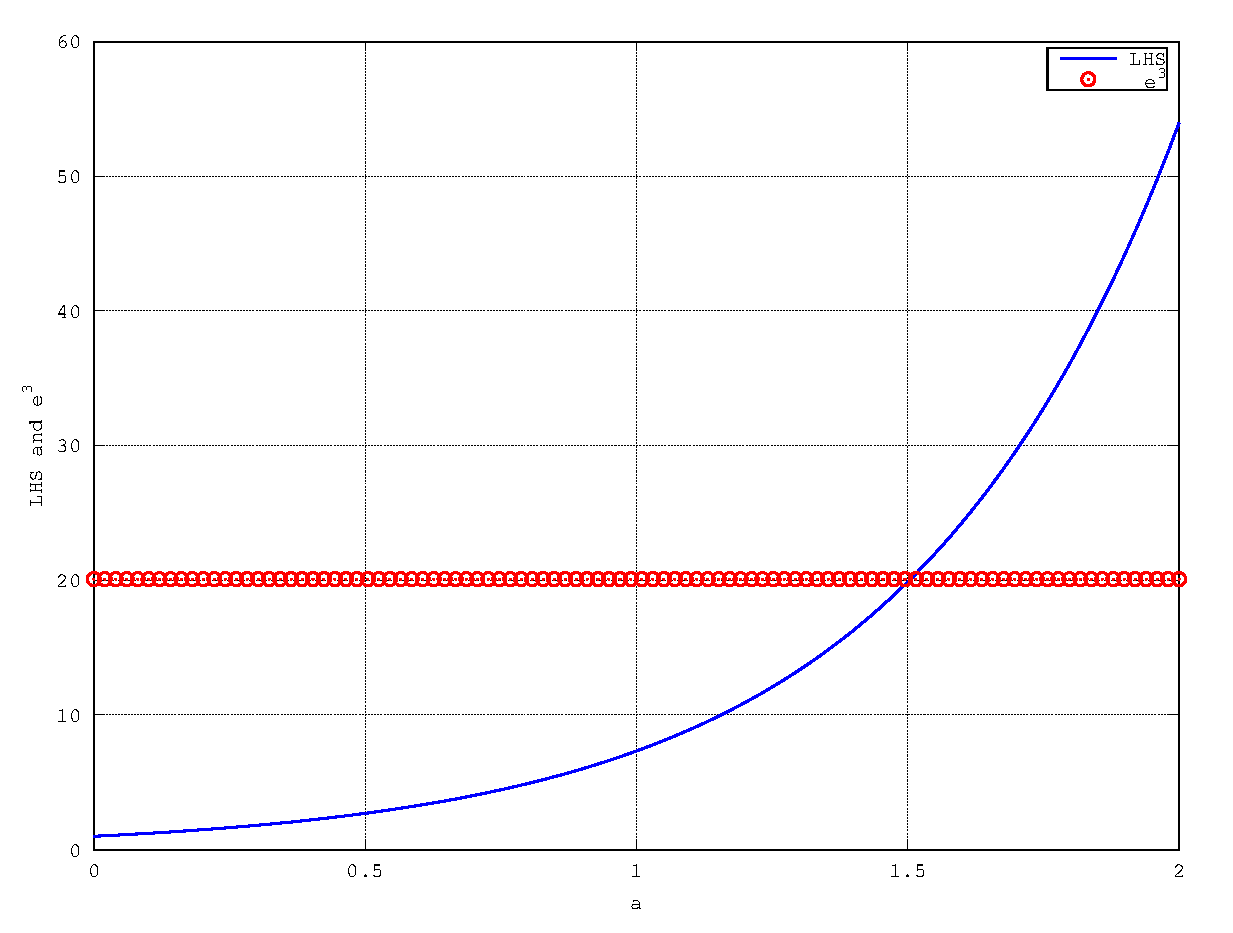
\includegraphics[width=\columnwidth]{./EE1083/pythonc/figs/ee16b1004}
%\end{center}
%\caption{LHS and RHS in \eqref{prob_four}}
%\label{fig:EE1083/pythonc/4}	
%\end{figure}

\bigskip
\fi

\begin{abstract}
This manual shows how to generate data in a file using a C program and importing it in Python.  
\end{abstract}
\begin{enumerate}
\item
Graphically show that the function
%
\begin{equation}
\label{eq:fx}
f(x)=
\begin{cases}
-x & x < 1 \\
a + \cos^{-1}\brak{x + b} & 1 \leq x \leq 2
\end{cases}
\end{equation}
%
is continuous at $x = 1$ for $b = -1, a - b =  - \frac{\pi}{2}$.  

\solution
%Since the function is differentiable at $x=1$,
\begin{align}
\label{four_one}
\lim _{ x\rightarrow { 1 }^{ - } }{ f^{ \prime  }\left( x \right)  }  &= \lim _{ x\rightarrow { 1 }^{ + } }{ f^{ \prime  }\left(x \right)  }
\end{align}
Also,
%
\begin{align}
\label{four_two}
 \lim _{ x\rightarrow { 1 }^{ - } }{ f^{ \prime  }\left( x \right)  } &=-1 \\ 
\lim _{ x\rightarrow { 1 }^{ + } }{ f^{ \prime  }\left(x \right)  } &= -\frac { 1 }{ \sqrt { 1-{ (x+b) }^{ 2 } }  } 
\end{align}
%
From \eqref{four_one} and \eqref{four_two},
\begin{align}
-\frac { 1 }{ \sqrt { 1-{ (x+b) }^{ 2 } }} &= -1 \Rightarrow 
b &=-x = -1
\end{align}
Since a differentiable function is also continuous, 
\begin{align}
\lim _{ x\rightarrow { 1 }^{ + } }{ \quad a+\cos ^{ -1 }{ (x+b) }  } &= \lim _{ x\rightarrow { 1 }^{ - } }{ (-x) }  \\
\Rightarrow a+\frac { \pi  }{ 2 } &=-1\\
\Rightarrow a &=-1-\frac { \pi  }{ 2 }
\end{align}
Then
\begin{align}
  c=\frac{a}{b}=1+\frac { \pi  }{ 2 } 
\end{align}


The following python code yields Fig. \ref{fig:EE1083/pythonc/5} verifying the above result.
\lstinputlisting[language=python]{./EE1083/pythonc/codes/ee16b1005.py}
\begin{figure}[!ht]
\begin{center}
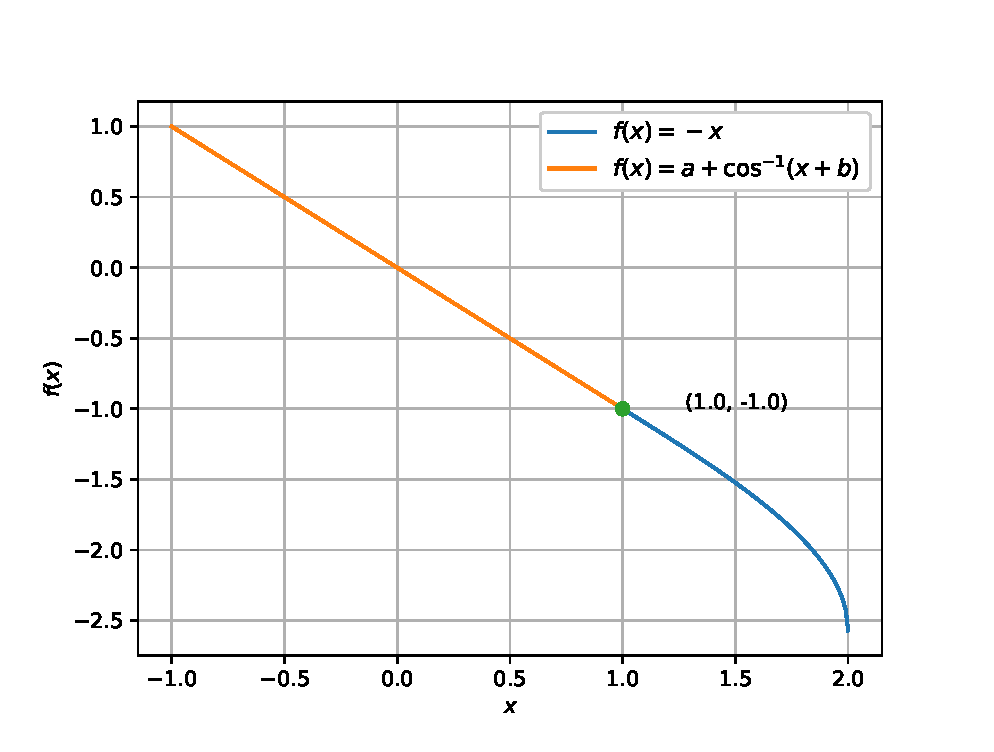
\includegraphics[width=\columnwidth]{./EE1083/pythonc/figs/ee16b1005}
\end{center}
\caption{Substituting the values of $a$ and $b$ in $f(x)$, the graph is smooth at $x=1$. So $f(x)$ is continuous as well as differentiable $x=1$.}
\label{fig:EE1083/pythonc/5}	
\end{figure}
%
\item
Write a C program to generate an arithmetic progression with first term $a=-1$, last term $l=1$ and number of terms $n=100$ and print the numbers on the screen.

\solution
\lstinputlisting[language=C]{./EE1083/pythonc/codes/ap.c}
\item
Repeat the above exercise by using functions for finding the common difference
and the $n$term given $a,l$ and $n$.

\solution
\lstinputlisting[language=C]{./EE1083/pythonc/codes/apfunc.c}
\item
Repeat the above exercise by printing the numbers in a file called test.dat

\solution
\lstinputlisting[language=C]{./EE1083/pythonc/codes/apfile.c}
\item
Now run the following program.  Comment.

\lstinputlisting[language=python]{./EE1083/pythonc/codes/ee16b1005_dat.py}
\item
Compute $f(x)$ in \eqref{eq:fx} through a C program

\solution
\lstinputlisting[language=C]{./EE1083/pythonc/codes/fx.c}
\item
Do all the computations in Problem 1 in C and verify your results by plotting in python.

\end{enumerate}
